% Created 2015-06-22 Mon 19:32
\documentclass[letterpaper, 9pt, onecolumn, twoside, technote, final]{IEEEtran}
\usepackage[utf8]{inputenc}
\usepackage[T1]{fontenc}
\usepackage{fixltx2e}
\usepackage{graphicx}
\usepackage{longtable}
\usepackage{float}
\usepackage{wrapfig}
\usepackage{rotating}
\usepackage[normalem]{ulem}
\usepackage{amsmath}
\usepackage{textcomp}
\usepackage{marvosym}
\usepackage{wasysym}
\usepackage{amssymb}
\usepackage{hyperref}
\tolerance=1000
\usepackage{minted}
\usepackage{minted}
\usepackage{makeidx}
\usepackage[lining,tabular]{fbb} % so math uses tabular lining figures
\usepackage[scaled=.95,type1]{cabin} % sans serif in style of Gill Sans
\usepackage[varqu,varl]{zi4}% inconsolata typewriter
\usepackage[T1]{fontenc} % LY1 also works
\usepackage[libertine,bigdelims]{newtxmath}
\usepackage[cal=boondoxo,bb=boondox,frak=boondox]{mathalfa}
\useosf % change normal text to use proportional oldstyle figures
\markboth{Reporte de gastos Febrero - Abril, 2015}%
{Sergio-Feliciano Mendoza-Barrera - CEO Global Labs Mexico}
\newcommand{\degC}{$^\circ$C{}}
\author{Sergio-Feliciano Mendoza-Barrera}
\date{20/06/2015}
\title{Homework Week 2}
\hypersetup{
  pdfkeywords={R, data science, emacs, ESS, org-mode},
  pdfsubject={R introduction, remembering the syntax and some useful examples},
  pdfcreator={Emacs 24.4.1 (Org mode 8.2.10)}}
\begin{document}

\maketitle

\begin{abstract}
Homework week 2.
\end{abstract}

\section{Climate Change [7/7]}
\label{sec-1}

There have been many studies documenting that the average global
temperature has been increasing over the last century. The
consequences of a continued rise in global temperature will be
dire. Rising sea levels and an increased frequency of extreme weather
events will affect billions of people.

In this problem, we will attempt to study the relationship between
average global temperature and several other factors.

The file \href{https://courses.edx.org/asset-v1:MITx\%2B15.071x_2a\%2B2T2015\%2Btype@asset\%2Bblock/climate_change.csv}{climate\_change.csv} contains climate data from \textbf{May 1983} to
\textbf{December 2008}. The available variables include:

\begin{itemize}
\item \textbf{Year}: the observation year.

\item \textbf{Month}: the observation month.

\item \textbf{Temp}: the difference in degrees Celsius between the average global
temperature in that period and a reference value. This data comes
from the \href{http://www.cru.uea.ac.uk/cru/data/temperature}{Climatic Research Unit at the University of East Anglia}.

\item \textbf{CO2, N2O, CH4, CFC.11, CFC.12}: atmospheric concentrations of carbon
dioxide (CO2), nitrous oxide (N2O), methane  (CH4),
trichlorofluoromethane (CCl3F; commonly referred to as CFC-11) and
dichlorodifluoromethane (CCl2F2; commonly referred to as CFC-12),
respectively. This data comes from the \href{http://www.esrl.noaa.gov/gmd/ccgg/data-products.html}{ESRL/NOAA Global Monitoring
Division}.

\begin{itemize}
\item \textbf{CO2, N2O and CH4} are expressed in ppmv (parts per million by
volume -- i.e., 397 ppmv of CO2 means that CO2 constitutes 397
millionths of the total volume of the atmosphere)
\item \textbf{CFC.11 and CFC.12} are expressed in ppbv (parts per billion by
volume).
\end{itemize}

\item \textbf{Aerosols}: the mean stratospheric aerosol optical depth at 550
nm. This variable is linked to volcanoes, as volcanic eruptions
result in new particles being added to the atmosphere, which affect
how much of the sun's energy is reflected back into space. This data
is from the \href{http://data.giss.nasa.gov/modelforce/strataer}{Godard Institute for Space Studies at NASA}.

\item \textbf{TSI}: the total solar irradiance (TSI) in $\frac{W}{m^2}$ (the rate
at which the sun's energy is deposited per unit area). Due to
sunspots and other solar phenomena, the amount of energy that is
given off by the sun varies substantially with time. This data is
from the \href{http://solarisheppa.geomar.de/solarisheppa/cmip5}{SOLARIS-HEPPA project website}.

\item \textbf{MEI}: multivariate El Nino Southern Oscillation index (MEI), a
measure of the strength of the \href{http://en.wikipedia.org/wiki/El_nino}{El Nino/La Nina-Southern Oscillation}
(a weather effect in the Pacific Ocean that affects global
temperatures). This data comes from the \href{http://www.esrl.noaa.gov/psd/enso/mei/table.html}{ESRL/NOAA Physical Sciences
Division}.
\end{itemize}

\subsection{{\bfseries\sffamily DONE} Problem 1.1 - Creating Our First Model (2 points possible)}
\label{sec-1-1}
We are interested in how changes in these variables affect future
temperatures, as well as how well these variables explain temperature
changes so far. To do this, first read the dataset climate\_change.csv
into R.

Then, split the data into a training set, consisting of all the
observations up to and including 2006, and a testing set consisting of
the remaining years (hint: use subset). A training set refers to the
data that will be used to build the model (this is the data we give to
the lm() function), and a testing set refers to the data we will use
to test our predictive ability.

\subsubsection{Download the data set}
\label{sec-1-1-1}

In this part we can download the data

\begin{minted}[]{r}
library(parallel)

if(!file.exists("../data")) {
        dir.create("../data")
}

fileUrl <-
        c("https://courses.edx.org/asset-v1:MITx+15.071x_2a+2T2015+type@asset+block/climate_change.csv")

fileName <- c("climate_change.csv")

dataPath <- "../data"

filePath <- paste(dataPath, fileName, sep = "/")

if(!file.exists(filePath)) {
        download.file(fileUrl, destfile = filePath, method = "curl")
}

list.files("../data")
\end{minted}

\begin{verbatim}
 [1] "AnonymityPoll.csv"      "baseball.csv"           "BoeingStock.csv"
 [4] "climate_change.csv"     "CocaColaStock.csv"      "CountryCodes.csv"
 [7] "CPSData.csv"            "FluTrain.csv"           "GEStock.csv"
[10] "IBMStock.csv"           "MetroAreaCodes.csv"     "mvtWeek1.csv"
[13] "NBA_test.csv"           "NBA_train.csv"          "pisa2009test.csv"
[16] "pisa2009train.csv"      "ProcterGambleStock.csv" "README.md"
[19] "USDA.csv"               "WHO.csv"                "WHO_Europe.csv"
[22] "wine.csv"               "wine_test.csv"
\end{verbatim}

\subsubsection{Loading the data}
\label{sec-1-1-2}

\begin{minted}[]{r}
writeLines("\n :: Read in data")
climateChange <- read.table("../data/climate_change.csv", sep = ",", header = TRUE)
str(climateChange)
summary(climateChange)
\end{minted}

\begin{verbatim}
 :: Read in data
'data.frame':	308 obs. of  11 variables:
 $ Year    : int  1983 1983 1983 1983 1983 1983 1983 1983 1984 1984 ...
 $ Month   : int  5 6 7 8 9 10 11 12 1 2 ...
 $ MEI     : num  2.556 2.167 1.741 1.13 0.428 ...
 $ CO2     : num  346 346 344 342 340 ...
 $ CH4     : num  1639 1634 1633 1631 1648 ...
 $ N2O     : num  304 304 304 304 304 ...
 $ CFC.11  : num  191 192 193 194 194 ...
 $ CFC.12  : num  350 352 354 356 357 ...
 $ TSI     : num  1366 1366 1366 1366 1366 ...
 $ Aerosols: num  0.0863 0.0794 0.0731 0.0673 0.0619 0.0569 0.0524 0.0486 0.0451 0.0416 ...
 $ Temp    : num  0.109 0.118 0.137 0.176 0.149 0.093 0.232 0.078 0.089 0.013 ...
      Year          Month             MEI               CO2
 Min.   :1983   Min.   : 1.000   Min.   :-1.6350   Min.   :340.2
 1st Qu.:1989   1st Qu.: 4.000   1st Qu.:-0.3987   1st Qu.:353.0
 Median :1996   Median : 7.000   Median : 0.2375   Median :361.7
 Mean   :1996   Mean   : 6.552   Mean   : 0.2756   Mean   :363.2
 3rd Qu.:2002   3rd Qu.:10.000   3rd Qu.: 0.8305   3rd Qu.:373.5
 Max.   :2008   Max.   :12.000   Max.   : 3.0010   Max.   :388.5
      CH4            N2O            CFC.11          CFC.12           TSI
 Min.   :1630   Min.   :303.7   Min.   :191.3   Min.   :350.1   Min.   :1365
 1st Qu.:1722   1st Qu.:308.1   1st Qu.:246.3   1st Qu.:472.4   1st Qu.:1366
 Median :1764   Median :311.5   Median :258.3   Median :528.4   Median :1366
 Mean   :1750   Mean   :312.4   Mean   :252.0   Mean   :497.5   Mean   :1366
 3rd Qu.:1787   3rd Qu.:317.0   3rd Qu.:267.0   3rd Qu.:540.5   3rd Qu.:1366
 Max.   :1814   Max.   :322.2   Max.   :271.5   Max.   :543.8   Max.   :1367
    Aerosols            Temp
 Min.   :0.00160   Min.   :-0.2820
 1st Qu.:0.00280   1st Qu.: 0.1217
 Median :0.00575   Median : 0.2480
 Mean   :0.01666   Mean   : 0.2568
 3rd Qu.:0.01260   3rd Qu.: 0.4073
 Max.   :0.14940   Max.   : 0.7390
\end{verbatim}

Splitting the data in two data sets for training and test data frames.

First data frame for training purposes:

\begin{minted}[]{r}
training <- subset(climateChange, Year <= 2006)

writeLines("\n :: Exploratory data analysis for the training dataframe")
str(training)
summary(training)
\end{minted}

\begin{verbatim}
 :: Exploratory data analysis for the training dataframe
'data.frame':	284 obs. of  11 variables:
 $ Year    : int  1983 1983 1983 1983 1983 1983 1983 1983 1984 1984 ...
 $ Month   : int  5 6 7 8 9 10 11 12 1 2 ...
 $ MEI     : num  2.556 2.167 1.741 1.13 0.428 ...
 $ CO2     : num  346 346 344 342 340 ...
 $ CH4     : num  1639 1634 1633 1631 1648 ...
 $ N2O     : num  304 304 304 304 304 ...
 $ CFC.11  : num  191 192 193 194 194 ...
 $ CFC.12  : num  350 352 354 356 357 ...
 $ TSI     : num  1366 1366 1366 1366 1366 ...
 $ Aerosols: num  0.0863 0.0794 0.0731 0.0673 0.0619 0.0569 0.0524 0.0486 0.0451 0.0416 ...
 $ Temp    : num  0.109 0.118 0.137 0.176 0.149 0.093 0.232 0.078 0.089 0.013 ...
      Year          Month             MEI               CO2
 Min.   :1983   Min.   : 1.000   Min.   :-1.5860   Min.   :340.2
 1st Qu.:1989   1st Qu.: 4.000   1st Qu.:-0.3230   1st Qu.:352.3
 Median :1995   Median : 7.000   Median : 0.3085   Median :359.9
 Mean   :1995   Mean   : 6.556   Mean   : 0.3419   Mean   :361.4
 3rd Qu.:2001   3rd Qu.:10.000   3rd Qu.: 0.8980   3rd Qu.:370.6
 Max.   :2006   Max.   :12.000   Max.   : 3.0010   Max.   :385.0
      CH4            N2O            CFC.11          CFC.12           TSI
 Min.   :1630   Min.   :303.7   Min.   :191.3   Min.   :350.1   Min.   :1365
 1st Qu.:1716   1st Qu.:307.7   1st Qu.:249.6   1st Qu.:462.5   1st Qu.:1366
 Median :1759   Median :310.8   Median :260.4   Median :522.1   Median :1366
 Mean   :1746   Mean   :311.7   Mean   :252.5   Mean   :494.2   Mean   :1366
 3rd Qu.:1782   3rd Qu.:316.1   3rd Qu.:267.4   3rd Qu.:541.0   3rd Qu.:1366
 Max.   :1808   Max.   :320.5   Max.   :271.5   Max.   :543.8   Max.   :1367
    Aerosols            Temp
 Min.   :0.00160   Min.   :-0.2820
 1st Qu.:0.00270   1st Qu.: 0.1180
 Median :0.00620   Median : 0.2325
 Mean   :0.01772   Mean   : 0.2478
 3rd Qu.:0.01400   3rd Qu.: 0.4065
 Max.   :0.14940   Max.   : 0.7390
\end{verbatim}

First data frame for test purposes:

\begin{minted}[]{r}
test <- subset(climateChange, Year > 2006)
str(test)
summary(test)
\end{minted}

\begin{verbatim}
'data.frame':	24 obs. of  11 variables:
 $ Year    : int  2007 2007 2007 2007 2007 2007 2007 2007 2007 2007 ...
 $ Month   : int  1 2 3 4 5 6 7 8 9 10 ...
 $ MEI     : num  0.974 0.51 0.074 -0.049 0.183 ...
 $ CO2     : num  383 384 385 386 387 ...
 $ CH4     : num  1800 1803 1803 1802 1796 ...
 $ N2O     : num  321 321 321 321 320 ...
 $ CFC.11  : num  248 248 248 248 247 ...
 $ CFC.12  : num  539 539 539 539 538 ...
 $ TSI     : num  1366 1366 1366 1366 1366 ...
 $ Aerosols: num  0.0054 0.0051 0.0045 0.0045 0.0041 0.004 0.004 0.0041 0.0042 0.0041 ...
 $ Temp    : num  0.601 0.498 0.435 0.466 0.372 0.382 0.394 0.358 0.402 0.362 ...
      Year          Month            MEI               CO2
 Min.   :2007   Min.   : 1.00   Min.   :-1.6350   Min.   :380.9
 1st Qu.:2007   1st Qu.: 3.75   1st Qu.:-1.0437   1st Qu.:383.1
 Median :2008   Median : 6.50   Median :-0.5305   Median :384.5
 Mean   :2008   Mean   : 6.50   Mean   :-0.5098   Mean   :384.7
 3rd Qu.:2008   3rd Qu.: 9.25   3rd Qu.:-0.0360   3rd Qu.:386.1
 Max.   :2008   Max.   :12.00   Max.   : 0.9740   Max.   :388.5
      CH4            N2O            CFC.11          CFC.12           TSI
 Min.   :1772   Min.   :320.3   Min.   :244.1   Min.   :534.9   Min.   :1366
 1st Qu.:1792   1st Qu.:320.6   1st Qu.:244.6   1st Qu.:535.1   1st Qu.:1366
 Median :1798   Median :321.3   Median :246.2   Median :537.0   Median :1366
 Mean   :1797   Mean   :321.1   Mean   :245.9   Mean   :536.7   Mean   :1366
 3rd Qu.:1804   3rd Qu.:321.4   3rd Qu.:246.6   3rd Qu.:537.4   3rd Qu.:1366
 Max.   :1814   Max.   :322.2   Max.   :248.4   Max.   :539.2   Max.   :1366
    Aerosols             Temp
 Min.   :0.003100   Min.   :0.074
 1st Qu.:0.003600   1st Qu.:0.307
 Median :0.004100   Median :0.380
 Mean   :0.004071   Mean   :0.363
 3rd Qu.:0.004500   3rd Qu.:0.414
 Max.   :0.005400   Max.   :0.601
\end{verbatim}

\subsubsection{Question a}
\label{sec-1-1-3}

Next, build a linear regression model to predict the dependent
variable Temp, using MEI, CO2, CH4, N2O, CFC.11, CFC.12, TSI, and
Aerosols as independent variables (Year and Month should NOT be used
in the model). Use the training set to build the model.

\begin{minted}[]{r}
writeLines("\n :: Linear regression model for Climate Change")
tempReg <- lm(Temp ~ MEI + CO2 + CH4 + N2O + CFC.11 + CFC.12 + TSI +
                      Aerosols, data = training)
summary(tempReg)
\end{minted}

\begin{verbatim}
 :: Linear regression model for Climate Change

Call:
lm(formula = Temp ~ MEI + CO2 + CH4 + N2O + CFC.11 + CFC.12 +
    TSI + Aerosols, data = training)

Residuals:
     Min       1Q   Median       3Q      Max
-0.25888 -0.05913 -0.00082  0.05649  0.32433

Coefficients:
              Estimate Std. Error t value Pr(>|t|)
(Intercept) -1.246e+02  1.989e+01  -6.265 1.43e-09 ***
MEI          6.421e-02  6.470e-03   9.923  < 2e-16 ***
CO2          6.457e-03  2.285e-03   2.826  0.00505 **
CH4          1.240e-04  5.158e-04   0.240  0.81015
N2O         -1.653e-02  8.565e-03  -1.930  0.05467 .
CFC.11      -6.631e-03  1.626e-03  -4.078 5.96e-05 ***
CFC.12       3.808e-03  1.014e-03   3.757  0.00021 ***
TSI          9.314e-02  1.475e-02   6.313 1.10e-09 ***
Aerosols    -1.538e+00  2.133e-01  -7.210 5.41e-12 ***
---
Signif. codes:  0 ‘***’ 0.001 ‘**’ 0.01 ‘*’ 0.05 ‘.’ 0.1 ‘ ’ 1

Residual standard error: 0.09171 on 275 degrees of freedom
Multiple R-squared:  0.7509,	Adjusted R-squared:  0.7436
F-statistic: 103.6 on 8 and 275 DF,  p-value: < 2.2e-16
\end{verbatim}

Enter the model R2 (the "Multiple R-squared" value):

\paragraph{Answer}
\label{sec-1-1-3-1}

0.7509

\textbf{Explanation}

First, read in the data and split it using the subset command:

climate = read.csv("climate\_change.csv")

train = subset(climate, Year <= 2006)

test = subset(climate, Year > 2006)

Then, you can create the model using the command:

climatelm = lm(Temp \textasciitilde{} MEI + CO2 + CH4 + N2O + CFC.11 + CFC.12 + TSI +
Aerosols, data=train)

Lastly, look at the model using summary(climatelm). The Multiple
R-squared value is 0.7509.

\subsection{{\bfseries\sffamily DONE} Problem 1.2 - Creating Our First Model (1 point possible)}
\label{sec-1-2}
Which variables are significant in the model? We will consider a
variable signficant only if the p-value is below 0.05. (Select all
that apply.)

\subsubsection{Answer}
\label{sec-1-2-1}

If you look at the model we created in the previous problem using
summary(climatelm), all of the variables have at least one star except
for CH4 and N2O. So MEI, CO2, CFC.11, CFC.12, TSI, and Aerosols are
all significant.

\subsection{{\bfseries\sffamily DONE} Problem 2.1 - Understanding the Model (1 point possible)}
\label{sec-1-3}
Current scientific opinion is that nitrous oxide and CFC-11 are
greenhouse gases: gases that are able to trap heat from the sun and
contribute to the heating of the Earth. However, the regression
coefficients of both the N2O and CFC-11 variables are negative,
indicating that increasing atmospheric concentrations of either of
these two compounds is associated with lower global temperatures.

Which of the following is the simplest correct explanation for this
contradiction?

\begin{minted}[]{r}
cor(training, use="complete.obs")
\end{minted}

\begin{verbatim}
                Year         Month           MEI         CO2         CH4
Year      1.00000000 -0.0279419602 -0.0369876842  0.98274939  0.91565945
Month    -0.02794196  1.0000000000  0.0008846905 -0.10673246  0.01856866
MEI      -0.03698768  0.0008846905  1.0000000000 -0.04114717 -0.03341930
CO2       0.98274939 -0.1067324607 -0.0411471651  1.00000000  0.87727963
CH4       0.91565945  0.0185686624 -0.0334193014  0.87727963  1.00000000
N2O       0.99384523  0.0136315303 -0.0508197755  0.97671982  0.89983864
CFC.11    0.56910643 -0.0131112236  0.0690004387  0.51405975  0.77990402
CFC.12    0.89701166  0.0006751102  0.0082855443  0.85268963  0.96361625
TSI       0.17030201 -0.0346061935 -0.1544919227  0.17742893  0.24552844
Aerosols -0.34524670  0.0148895406  0.3402377871 -0.35615480 -0.26780919
Temp      0.78679714 -0.0998567411  0.1724707512  0.78852921  0.70325502
                 N2O      CFC.11        CFC.12         TSI    Aerosols
Year      0.99384523  0.56910643  0.8970116635  0.17030201 -0.34524670
Month     0.01363153 -0.01311122  0.0006751102 -0.03460619  0.01488954
MEI      -0.05081978  0.06900044  0.0082855443 -0.15449192  0.34023779
CO2       0.97671982  0.51405975  0.8526896272  0.17742893 -0.35615480
CH4       0.89983864  0.77990402  0.9636162478  0.24552844 -0.26780919
N2O       1.00000000  0.52247732  0.8679307757  0.19975668 -0.33705457
CFC.11    0.52247732  1.00000000  0.8689851828  0.27204596 -0.04392120
CFC.12    0.86793078  0.86898518  1.0000000000  0.25530281 -0.22513124
TSI       0.19975668  0.27204596  0.2553028138  1.00000000  0.05211651
Aerosols -0.33705457 -0.04392120 -0.2251312440  0.05211651  1.00000000
Temp      0.77863893  0.40771029  0.6875575483  0.24338269 -0.38491375
                Temp
Year      0.78679714
Month    -0.09985674
MEI       0.17247075
CO2       0.78852921
CH4       0.70325502
N2O       0.77863893
CFC.11    0.40771029
CFC.12    0.68755755
TSI       0.24338269
Aerosols -0.38491375
Temp      1.00000000
\end{verbatim}

\begin{figure}[htb]
\centering
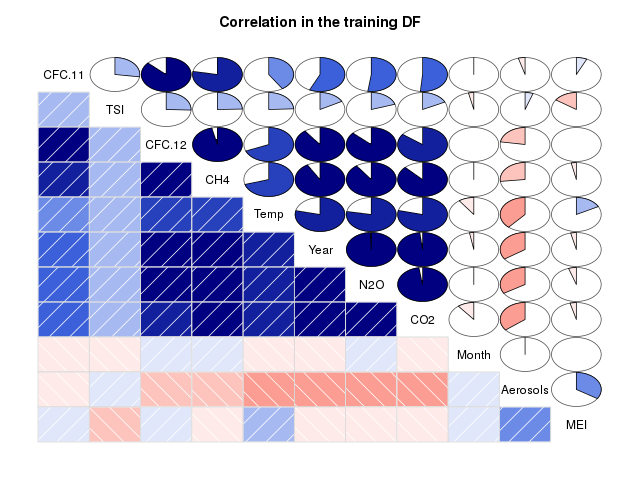
\includegraphics[width=.9\linewidth]{../graphs/climateChangeVarCorr.png}
\caption{\label{fig:climateChangeVarCorr}Correlation plot of the climate change variables}
\end{figure}

The correlation plot shows a strong correlation between $N_2 O$ and
and $CO_2$ in one hand, in other hand $CFC.11$ is highly correlated
with $CFC.12$ and $CH_4$.

\subsubsection{Answer}
\label{sec-1-3-1}

The linear correlation of N2O and CFC.11 with other variables in the
data set is quite large. The first explanation does not seem correct,
as the warming effect of nitrous oxide and CFC-11 are well documented,
and our regression analysis is not enough to disprove it. The second
explanation is unlikely, as we have estimated eight coefficients and
the intercept from 284 observations.

\subsection{{\bfseries\sffamily DONE} Problem 2.2 - Understanding the Model (2 points possible)}
\label{sec-1-4}
Compute the correlations between all the variables in the training
set.

\subsubsection{Question a}
\label{sec-1-4-1}

Which of the following independent variables is $N_2O$ highly correlated
with (absolute correlation greater than 0.7)? Select all that apply.

\paragraph{Answer}
\label{sec-1-4-1-1}

CO2
CH4
CFC.12

\subsubsection{Question b}
\label{sec-1-4-2}

Which of the following independent variables is $CFC.11$ highly
correlated with? Select all that apply.

CH4
CFC.12

\textbf{Explanation}

You can calculate all correlations at once using cor(train) where
train is the name of the training data set.

\subsection{{\bfseries\sffamily DONE} Problem 3 - Simplifying the Model (2 points possible)}
\label{sec-1-5}
Given that the correlations are so high, let us focus on the $N_2O$
variable and build a model with only MEI, TSI, Aerosols and $N_2O$ as
independent variables. Remember to use the training set to build the
model.

\begin{minted}[]{r}
writeLines("\n :: Linear regression model for Climate Change")
tempReg2 <- lm(Temp ~ MEI + TSI + Aerosols + N2O, data = training)
summary(tempReg2)
\end{minted}

\begin{verbatim}
 null device
          1

 :: Linear regression model for Climate Change

Call:
lm(formula = Temp ~ MEI + TSI + Aerosols + N2O, data = training)

Residuals:
     Min       1Q   Median       3Q      Max
-0.27916 -0.05975 -0.00595  0.05672  0.34195

Coefficients:
              Estimate Std. Error t value Pr(>|t|)
(Intercept) -1.162e+02  2.022e+01  -5.747 2.37e-08 ***
MEI          6.419e-02  6.652e-03   9.649  < 2e-16 ***
TSI          7.949e-02  1.487e-02   5.344 1.89e-07 ***
Aerosols    -1.702e+00  2.180e-01  -7.806 1.19e-13 ***
N2O          2.532e-02  1.311e-03  19.307  < 2e-16 ***
---
Signif. codes:  0 ‘***’ 0.001 ‘**’ 0.01 ‘*’ 0.05 ‘.’ 0.1 ‘ ’ 1

Residual standard error: 0.09547 on 279 degrees of freedom
Multiple R-squared:  0.7261,	Adjusted R-squared:  0.7222
F-statistic: 184.9 on 4 and 279 DF,  p-value: < 2.2e-16
\end{verbatim}

\subsubsection{Question a}
\label{sec-1-5-1}

Enter the coefficient of $N_2O$ in this reduced model:

\paragraph{Answer}
\label{sec-1-5-1-1}

2.532e-02

\subsubsection{Question b}
\label{sec-1-5-2}

(How does this compare to the coefficient in the previous model with
all of the variables?)

Enter the model $R^2$:

\paragraph{Answer}
\label{sec-1-5-2-1}

0.7261

\textbf{Explanation}

We can create this simplified model with the command:

LinReg = lm(Temp \textasciitilde{} MEI + N2O + TSI + Aerosols, data=train)

You can get the coefficient for N2O and the model R-squared by typing
summary(LinReg).

We have observed that, for this problem, when we remove many variables
the sign of N2O flips. The model has not lost a lot of explanatory
power (the model R2 is 0.7261 compared to 0.7509 previously) despite
removing many variables. As discussed in lecture, this type of
behavior is typical when building a model where many of the
independent variables are highly correlated with each other. In this
particular problem many of the variables (CO2, CH4, N2O, CFC.11 and
CFC.12) are highly correlated, since they are all driven by human
industrial development.

\subsection{{\bfseries\sffamily DONE} Problem 4 - Automatically Building the Model (4 points possible)}
\label{sec-1-6}
We have many variables in this problem, and as we have seen above,
dropping some from the model does not decrease model quality. R
provides a function, step, that will automate the procedure of trying
different combinations of variables to find a good compromise of model
simplicity and $R^2$. This trade-off is formalized by the \textbf{Akaike}
information criterion (\href{http://en.wikipedia.org/wiki/Akaike_information_criterion}{AIC}) - it can be informally thought of as the
quality of the model with a penalty for the number of variables in the
model.

The step function has one argument - the name of the initial model. It
returns a simplified model. Use the step function in R to derive a new
model, with the full model as the initial model (HINT: If your initial
full model was called "climateLM", you could create a new model with
the step function by typing step(climateLM). Be sure to save your new
model to a variable name so that you can look at the summary. For more
information about the step function, type ?step in your R console.)

\begin{minted}[]{r}
writeLines("\n :: Optimizing the linear regression model for Climate Change")
tempReg3 <- step(tempReg)
summary(tempReg3)
\end{minted}

\begin{verbatim}
 :: Optimizing the linear regression model for Climate Change
Start:  AIC=-1348.16
Temp ~ MEI + CO2 + CH4 + N2O + CFC.11 + CFC.12 + TSI + Aerosols

           Df Sum of Sq    RSS     AIC
- CH4       1   0.00049 2.3135 -1350.1
<none>                  2.3130 -1348.2
- N2O       1   0.03132 2.3443 -1346.3
- CO2       1   0.06719 2.3802 -1342.0
- CFC.12    1   0.11874 2.4318 -1335.9
- CFC.11    1   0.13986 2.4529 -1333.5
- TSI       1   0.33516 2.6482 -1311.7
- Aerosols  1   0.43727 2.7503 -1301.0
- MEI       1   0.82823 3.1412 -1263.2

Step:  AIC=-1350.1
Temp ~ MEI + CO2 + N2O + CFC.11 + CFC.12 + TSI + Aerosols

           Df Sum of Sq    RSS     AIC
<none>                  2.3135 -1350.1
- N2O       1   0.03133 2.3448 -1348.3
- CO2       1   0.06672 2.3802 -1344.0
- CFC.12    1   0.13023 2.4437 -1336.5
- CFC.11    1   0.13938 2.4529 -1335.5
- TSI       1   0.33500 2.6485 -1313.7
- Aerosols  1   0.43987 2.7534 -1302.7
- MEI       1   0.83118 3.1447 -1264.9

Call:
lm(formula = Temp ~ MEI + CO2 + N2O + CFC.11 + CFC.12 + TSI +
    Aerosols, data = training)

Residuals:
     Min       1Q   Median       3Q      Max
-0.25770 -0.05994 -0.00104  0.05588  0.32203

Coefficients:
              Estimate Std. Error t value Pr(>|t|)
(Intercept) -1.245e+02  1.985e+01  -6.273 1.37e-09 ***
MEI          6.407e-02  6.434e-03   9.958  < 2e-16 ***
CO2          6.402e-03  2.269e-03   2.821 0.005129 **
N2O         -1.602e-02  8.287e-03  -1.933 0.054234 .
CFC.11      -6.609e-03  1.621e-03  -4.078 5.95e-05 ***
CFC.12       3.868e-03  9.812e-04   3.942 0.000103 ***
TSI          9.312e-02  1.473e-02   6.322 1.04e-09 ***
Aerosols    -1.540e+00  2.126e-01  -7.244 4.36e-12 ***
---
Signif. codes:  0 ‘***’ 0.001 ‘**’ 0.01 ‘*’ 0.05 ‘.’ 0.1 ‘ ’ 1

Residual standard error: 0.09155 on 276 degrees of freedom
Multiple R-squared:  0.7508,	Adjusted R-squared:  0.7445
F-statistic: 118.8 on 7 and 276 DF,  p-value: < 2.2e-16
\end{verbatim}

\subsubsection{Question a}
\label{sec-1-6-1}

Enter the R2 value of the model produced by the step function:

\paragraph{Answer}
\label{sec-1-6-1-1}

\textbf{Only $CH_4$ was removed}.

It is interesting to note that the step function does not address the
collinearity of the variables, except that adding highly correlated
variables will not improve the R2 significantly. The consequence of
this is that the step function will not necessarily produce a very
interpretable model - just a model that has balanced quality and
simplicity for a particular weighting of quality and simplicity
(AIC).

\subsection{{\bfseries\sffamily DONE} Problem 5 - Testing on Unseen Data (2 points possible)}
\label{sec-1-7}
We have developed an understanding of how well we can fit a linear
regression to the training data, but does the model quality hold when
applied to unseen data?

Using the model produced from the step function, calculate temperature
predictions for the testing data set, using the predict function.

\begin{minted}[]{r}
writeLines("\n :: Make test set predictions")
predictTest <- predict(tempReg3, newdata = test)
predictTest
\end{minted}

\begin{verbatim}

 :: Make test set predictions
      285       286       287       288       289       290       291       292
0.4677808 0.4435404 0.4265541 0.4299162 0.4455113 0.4151422 0.4097367 0.3839390
      293       294       295       296       297       298       299       300
0.3255595 0.3274147 0.3231401 0.3316704 0.3522134 0.3313129 0.3142112 0.3703410
      301       302       303       304       305       306       307       308
0.4162213 0.4391458 0.4237965 0.3913679 0.3587615 0.3451991 0.3607087 0.3638076
\end{verbatim}

But to get a measure of the predictions goodness of fit, we need to
calculate the \textbf{out of sample R-squared}.

\begin{minted}[]{r}
writeLines("\n :: Compute out-of-sample R^2")
SSE <- sum((predictTest - test$Temp)^2)
SST <- sum((mean(training$Temp) - test$Temp)^2)
R2 <- 1 - (SSE/SST)
R2
\end{minted}

\begin{verbatim}

 :: Compute out-of-sample R^2
[1] 0.6286051
\end{verbatim}

Enter the testing set R2:

\subsubsection{Answer}
\label{sec-1-7-1}

0.6286051

\textbf{Explanation}

The R code to calculate the R-squared can be written as follows (your
variable names may be different):

tempPredict = predict(climateStep, newdata = test)

SSE = sum((tempPredict - test\$Temp)\^{}2)

SST = sum( (mean(train\$Temp) - test\$Temp)\^{}2)

R2 = 1 - SSE/SST

\section{Reading Test Scores [16/16]}
\label{sec-2}

The Programme for International Student Assessment (PISA) is a test
given every three years to 15-year-old students from around the world
to evaluate their performance in mathematics, reading, and
science. This test provides a quantitative way to compare the
performance of students from different parts of the world. In this
homework assignment, we will predict the reading scores of students
from the United States of America on the 2009 PISA exam.

The datasets \href{https://courses.edx.org/asset-v1:MITx\%2B15.071x_2a\%2B2T2015\%2Btype@asset\%2Bblock/pisa2009train.csv}{pisa2009train.csv} and \href{https://courses.edx.org/asset-v1:MITx\%2B15.071x_2a\%2B2T2015\%2Btype@asset\%2Bblock/pisa2009test.csv}{pisa2009test.csv} contain
information about the demographics and schools for American students
taking the exam, derived from \href{http://nces.ed.gov/pubsearch/pubsinfo.asp?pubid\%3D2011038}{2009 PISA Public-Use Data Files}
distributed by the United States National Center for Education
Statistics (NCES). While the datasets are not supposed to contain
identifying information about students taking the test, by using the
data you are bound by the \href{https://courses.edx.org/asset-v1:MITx\%2B15.071x_2a\%2B2T2015\%2Btype@asset\%2Bblock/NCES_Data_Use_Agreement.txt}{NCES data use agreement}, which prohibits any
attempt to determine the identity of any student in the datasets.

Each row in the datasets pisa2009train.csv and pisa2009test.csv
represents one student taking the exam. The datasets have the
following variables:

\begin{itemize}
\item \textbf{grade}: The grade in school of the student (most 15-year-olds in
America are in 10th grade)

\item \textbf{male}: Whether the student is male (1/0)

\item \textbf{raceeth}: The race/ethnicity composite of the student

\item \textbf{preschool}: Whether the student attended preschool (1/0)

\item \textbf{expectBachelors}: Whether the student expects to obtain a
bachelor's degree (1/0)

\item \textbf{motherHS}: Whether the student's mother completed high school (1/0)

\item \textbf{motherBachelors}: Whether the student's mother obtained a
bachelor's degree (1/0)

\item \textbf{motherWork}: Whether the student's mother has part-time or
full-time work (1/0)

\item \textbf{fatherHS}: Whether the student's father completed high school (1/0)

\item \textbf{fatherBachelors}: Whether the student's father obtained a
bachelor's degree (1/0)

\item \textbf{fatherWork}: Whether the student's father has part-time or
full-time work (1/0)

\item \textbf{selfBornUS}: Whether the student was born in the United States of
America (1/0)

\item \textbf{motherBornUS}: Whether the student's mother was born in the United
States of America (1/0)

\item \textbf{fatherBornUS}: Whether the student's father was born in the United
States of America (1/0)

\item \textbf{englishAtHome}: Whether the student speaks English at home (1/0)

\item \textbf{computerForSchoolwork}: Whether the student has access to a
computer for schoolwork (1/0)

\item \textbf{read30MinsADay}: Whether the student reads for pleasure for 30
minutes/day (1/0)

\item \textbf{minutesPerWeekEnglish}: The number of minutes per week the student
spend in English class

\item \textbf{studentsInEnglish}: The number of students in this student's
English class at school

\item \textbf{schoolHasLibrary}: Whether this student's school has a library
(1/0)

\item \textbf{publicSchool}: Whether this student attends a public school (1/0)

\item \textbf{urban}: Whether this student's school is in an urban area (1/0)

\item \textbf{schoolSize}: The number of students in this student's school

\item \textbf{readingScore}: The student's reading score, on a 1000-point scale
\end{itemize}

\subsection{{\bfseries\sffamily DONE} Problem 1.1 - Dataset size (1 point possible)}
\label{sec-2-1}
Load the training and testing sets using the read.csv() function, and
save them as variables with the names pisaTrain and pisaTest.

\subsubsection{Download the data sets}
\label{sec-2-1-1}

In this part we can download the data

\begin{minted}[]{r}
library(parallel)

if(!file.exists("../data")) {
        dir.create("../data")
}

fileUrl <-
        c("https://courses.edx.org/asset-v1:MITx+15.071x_2a+2T2015+type@asset+block/pisa2009train.csv", "https://courses.edx.org/asset-v1:MITx+15.071x_2a+2T2015+type@asset+block/pisa2009test.csv")

fileName <- c("pisa2009train.csv", "pisa2009test.csv")

dataPath <- "../data"

for(i in 1:2) {
        filePath <- paste(dataPath, fileName[i], sep = "/")

        if(!file.exists(filePath)) {
                download.file(fileUrl[i], destfile = filePath, method = "curl")
        }
}
list.files("../data")
\end{minted}

\begin{verbatim}
 [1] "AnonymityPoll.csv"      "baseball.csv"           "BoeingStock.csv"
 [4] "climate_change.csv"     "CocaColaStock.csv"      "CountryCodes.csv"
 [7] "CPSData.csv"            "FluTrain.csv"           "GEStock.csv"
[10] "IBMStock.csv"           "MetroAreaCodes.csv"     "mvtWeek1.csv"
[13] "NBA_test.csv"           "NBA_train.csv"          "pisa2009test.csv"
[16] "pisa2009train.csv"      "ProcterGambleStock.csv" "README.md"
[19] "USDA.csv"               "WHO.csv"                "WHO_Europe.csv"
[22] "wine.csv"               "wine_test.csv"
\end{verbatim}

\subsubsection{Loading the data}
\label{sec-2-1-2}

\begin{minted}[]{r}
writeLines("\n :: Read the training data set")
pisaTrain <- read.table("../data/pisa2009train.csv", sep = ",", header = TRUE)
str(pisaTrain)
summary(pisaTrain)

writeLines("\n\n :: Read the test data set: DO NOT SEE THE DATA!")
pisaTest <- read.table("../data/pisa2009test.csv", sep = ",", header = TRUE)
\end{minted}

\begin{verbatim}
 :: Read the training data set
'data.frame':	3663 obs. of  24 variables:
 $ grade                : int  11 11 9 10 10 10 10 10 9 10 ...
 $ male                 : int  1 1 1 0 1 1 0 0 0 1 ...
 $ raceeth              : Factor w/ 7 levels "American Indian/Alaska Native",..: NA 7 7 3 4 3 2 7 7 5 ...
 $ preschool            : int  NA 0 1 1 1 1 0 1 1 1 ...
 $ expectBachelors      : int  0 0 1 1 0 1 1 1 0 1 ...
 $ motherHS             : int  NA 1 1 0 1 NA 1 1 1 1 ...
 $ motherBachelors      : int  NA 1 1 0 0 NA 0 0 NA 1 ...
 $ motherWork           : int  1 1 1 1 1 1 1 0 1 1 ...
 $ fatherHS             : int  NA 1 1 1 1 1 NA 1 0 0 ...
 $ fatherBachelors      : int  NA 0 NA 0 0 0 NA 0 NA 0 ...
 $ fatherWork           : int  1 1 1 1 0 1 NA 1 1 1 ...
 $ selfBornUS           : int  1 1 1 1 1 1 0 1 1 1 ...
 $ motherBornUS         : int  0 1 1 1 1 1 1 1 1 1 ...
 $ fatherBornUS         : int  0 1 1 1 0 1 NA 1 1 1 ...
 $ englishAtHome        : int  0 1 1 1 1 1 1 1 1 1 ...
 $ computerForSchoolwork: int  1 1 1 1 1 1 1 1 1 1 ...
 $ read30MinsADay       : int  0 1 0 1 1 0 0 1 0 0 ...
 $ minutesPerWeekEnglish: int  225 450 250 200 250 300 250 300 378 294 ...
 $ studentsInEnglish    : int  NA 25 28 23 35 20 28 30 20 24 ...
 $ schoolHasLibrary     : int  1 1 1 1 1 1 1 1 0 1 ...
 $ publicSchool         : int  1 1 1 1 1 1 1 1 1 1 ...
 $ urban                : int  1 0 0 1 1 0 1 0 1 0 ...
 $ schoolSize           : int  673 1173 1233 2640 1095 227 2080 1913 502 899 ...
 $ readingScore         : num  476 575 555 458 614 ...
     grade            male                      raceeth       preschool
 Min.   : 8.00   Min.   :0.0000   White             :2015   Min.   :0.0000
 1st Qu.:10.00   1st Qu.:0.0000   Hispanic          : 834   1st Qu.:0.0000
 Median :10.00   Median :1.0000   Black             : 444   Median :1.0000
 Mean   :10.09   Mean   :0.5111   Asian             : 143   Mean   :0.7228
 3rd Qu.:10.00   3rd Qu.:1.0000   More than one race: 124   3rd Qu.:1.0000
 Max.   :12.00   Max.   :1.0000   (Other)           :  68   Max.   :1.0000
                                  NA's              :  35   NA's   :56
 expectBachelors     motherHS    motherBachelors    motherWork
 Min.   :0.0000   Min.   :0.00   Min.   :0.0000   Min.   :0.0000
 1st Qu.:1.0000   1st Qu.:1.00   1st Qu.:0.0000   1st Qu.:0.0000
 Median :1.0000   Median :1.00   Median :0.0000   Median :1.0000
 Mean   :0.7859   Mean   :0.88   Mean   :0.3481   Mean   :0.7345
 3rd Qu.:1.0000   3rd Qu.:1.00   3rd Qu.:1.0000   3rd Qu.:1.0000
 Max.   :1.0000   Max.   :1.00   Max.   :1.0000   Max.   :1.0000
 NA's   :62       NA's   :97     NA's   :397      NA's   :93
    fatherHS      fatherBachelors    fatherWork       selfBornUS
 Min.   :0.0000   Min.   :0.0000   Min.   :0.0000   Min.   :0.0000
 1st Qu.:1.0000   1st Qu.:0.0000   1st Qu.:1.0000   1st Qu.:1.0000
 Median :1.0000   Median :0.0000   Median :1.0000   Median :1.0000
 Mean   :0.8593   Mean   :0.3319   Mean   :0.8531   Mean   :0.9313
 3rd Qu.:1.0000   3rd Qu.:1.0000   3rd Qu.:1.0000   3rd Qu.:1.0000
 Max.   :1.0000   Max.   :1.0000   Max.   :1.0000   Max.   :1.0000
 NA's   :245      NA's   :569      NA's   :233      NA's   :69
  motherBornUS     fatherBornUS    englishAtHome    computerForSchoolwork
 Min.   :0.0000   Min.   :0.0000   Min.   :0.0000   Min.   :0.0000
 1st Qu.:1.0000   1st Qu.:1.0000   1st Qu.:1.0000   1st Qu.:1.0000
 Median :1.0000   Median :1.0000   Median :1.0000   Median :1.0000
 Mean   :0.7725   Mean   :0.7668   Mean   :0.8717   Mean   :0.8994
 3rd Qu.:1.0000   3rd Qu.:1.0000   3rd Qu.:1.0000   3rd Qu.:1.0000
 Max.   :1.0000   Max.   :1.0000   Max.   :1.0000   Max.   :1.0000
 NA's   :71       NA's   :113      NA's   :71       NA's   :65
 read30MinsADay   minutesPerWeekEnglish studentsInEnglish schoolHasLibrary
 Min.   :0.0000   Min.   :   0.0        Min.   : 1.0      Min.   :0.0000
 1st Qu.:0.0000   1st Qu.: 225.0        1st Qu.:20.0      1st Qu.:1.0000
 Median :0.0000   Median : 250.0        Median :25.0      Median :1.0000
 Mean   :0.2899   Mean   : 266.2        Mean   :24.5      Mean   :0.9676
 3rd Qu.:1.0000   3rd Qu.: 300.0        3rd Qu.:30.0      3rd Qu.:1.0000
 Max.   :1.0000   Max.   :2400.0        Max.   :75.0      Max.   :1.0000
 NA's   :34       NA's   :186           NA's   :249       NA's   :143
  publicSchool        urban          schoolSize    readingScore
 Min.   :0.0000   Min.   :0.0000   Min.   : 100   Min.   :168.6
 1st Qu.:1.0000   1st Qu.:0.0000   1st Qu.: 712   1st Qu.:431.7
 Median :1.0000   Median :0.0000   Median :1212   Median :499.7
 Mean   :0.9339   Mean   :0.3849   Mean   :1369   Mean   :497.9
 3rd Qu.:1.0000   3rd Qu.:1.0000   3rd Qu.:1900   3rd Qu.:566.2
 Max.   :1.0000   Max.   :1.0000   Max.   :6694   Max.   :746.0
                                   NA's   :162


 :: Read the test data set: DO NOT SEE THE DATA!
\end{verbatim}

\subsubsection{Question a}
\label{sec-2-1-3}

How many students are there in the training set?

\paragraph{Answer}
\label{sec-2-1-3-1}

\begin{minted}[]{r}
writeLines("\n :: Number of students in the training data set")
nrow(pisaTrain)
\end{minted}

\begin{verbatim}

 :: Number of students in the training data set
[1] 3663
\end{verbatim}

\textbf{Explanation}

The datasets can be loaded with:

pisaTrain = read.csv("pisa2009train.csv")

pisaTest = read.csv("pisa2009test.csv")

We can then access the number of rows in the training set with
str(pisaTrain) or nrow(pisaTrain).

\subsection{{\bfseries\sffamily DONE} Problem 1.2 - Summarizing the dataset (2 points possible)}
\label{sec-2-2}
Using tapply() on pisaTrain, what is the average reading test score of
males?

\begin{minted}[]{r}
tapply(pisaTrain$readingScore, pisaTrain$male, mean)
\end{minted}

\begin{verbatim}
       0        1
512.9406 483.5325
\end{verbatim}

\subsubsection{Answer}
\label{sec-2-2-1}

The correct invocation of tapply() here is:

tapply(pisaTrain\$readingScore, pisaTrain\$male, mean)

\begin{center}
\begin{tabular}{ll}
Females & Males\\
\hline
$512.9406$ & $483.5325$\\
\end{tabular}
\end{center}

\subsection{{\bfseries\sffamily DONE} Problem 1.3 - Locating missing values (1 point possible)}
\label{sec-2-3}
Which variables are missing data in at least one observation in the
training set? Select all that apply.

\begin{minted}[]{r}
writeLines("\n :: any NA in the features")
summary(pisaTrain)
\end{minted}

\begin{verbatim}
:: any NA in the features
    grade            male                      raceeth       preschool
Min.   : 8.00   Min.   :0.0000   White             :2015   Min.   :0.0000
1st Qu.:10.00   1st Qu.:0.0000   Hispanic          : 834   1st Qu.:0.0000
Median :10.00   Median :1.0000   Black             : 444   Median :1.0000
Mean   :10.09   Mean   :0.5111   Asian             : 143   Mean   :0.7228
3rd Qu.:10.00   3rd Qu.:1.0000   More than one race: 124   3rd Qu.:1.0000
Max.   :12.00   Max.   :1.0000   (Other)           :  68   Max.   :1.0000
                                 NA's              :  35   NA's   :56
expectBachelors     motherHS    motherBachelors    motherWork
Min.   :0.0000   Min.   :0.00   Min.   :0.0000   Min.   :0.0000
1st Qu.:1.0000   1st Qu.:1.00   1st Qu.:0.0000   1st Qu.:0.0000
Median :1.0000   Median :1.00   Median :0.0000   Median :1.0000
Mean   :0.7859   Mean   :0.88   Mean   :0.3481   Mean   :0.7345
3rd Qu.:1.0000   3rd Qu.:1.00   3rd Qu.:1.0000   3rd Qu.:1.0000
Max.   :1.0000   Max.   :1.00   Max.   :1.0000   Max.   :1.0000
NA's   :62       NA's   :97     NA's   :397      NA's   :93
   fatherHS      fatherBachelors    fatherWork       selfBornUS
Min.   :0.0000   Min.   :0.0000   Min.   :0.0000   Min.   :0.0000
1st Qu.:1.0000   1st Qu.:0.0000   1st Qu.:1.0000   1st Qu.:1.0000
Median :1.0000   Median :0.0000   Median :1.0000   Median :1.0000
Mean   :0.8593   Mean   :0.3319   Mean   :0.8531   Mean   :0.9313
3rd Qu.:1.0000   3rd Qu.:1.0000   3rd Qu.:1.0000   3rd Qu.:1.0000
Max.   :1.0000   Max.   :1.0000   Max.   :1.0000   Max.   :1.0000
NA's   :245      NA's   :569      NA's   :233      NA's   :69
 motherBornUS     fatherBornUS    englishAtHome    computerForSchoolwork
Min.   :0.0000   Min.   :0.0000   Min.   :0.0000   Min.   :0.0000
1st Qu.:1.0000   1st Qu.:1.0000   1st Qu.:1.0000   1st Qu.:1.0000
Median :1.0000   Median :1.0000   Median :1.0000   Median :1.0000
Mean   :0.7725   Mean   :0.7668   Mean   :0.8717   Mean   :0.8994
3rd Qu.:1.0000   3rd Qu.:1.0000   3rd Qu.:1.0000   3rd Qu.:1.0000
Max.   :1.0000   Max.   :1.0000   Max.   :1.0000   Max.   :1.0000
NA's   :71       NA's   :113      NA's   :71       NA's   :65
read30MinsADay   minutesPerWeekEnglish studentsInEnglish schoolHasLibrary
Min.   :0.0000   Min.   :   0.0        Min.   : 1.0      Min.   :0.0000
1st Qu.:0.0000   1st Qu.: 225.0        1st Qu.:20.0      1st Qu.:1.0000
Median :0.0000   Median : 250.0        Median :25.0      Median :1.0000
Mean   :0.2899   Mean   : 266.2        Mean   :24.5      Mean   :0.9676
3rd Qu.:1.0000   3rd Qu.: 300.0        3rd Qu.:30.0      3rd Qu.:1.0000
Max.   :1.0000   Max.   :2400.0        Max.   :75.0      Max.   :1.0000
NA's   :34       NA's   :186           NA's   :249       NA's   :143
 publicSchool        urban          schoolSize    readingScore
Min.   :0.0000   Min.   :0.0000   Min.   : 100   Min.   :168.6
1st Qu.:1.0000   1st Qu.:0.0000   1st Qu.: 712   1st Qu.:431.7
Median :1.0000   Median :0.0000   Median :1212   Median :499.7
Mean   :0.9339   Mean   :0.3849   Mean   :1369   Mean   :497.9
3rd Qu.:1.0000   3rd Qu.:1.0000   3rd Qu.:1900   3rd Qu.:566.2
Max.   :1.0000   Max.   :1.0000   Max.   :6694   Max.   :746.0
                                  NA's   :162
\end{verbatim}

\subsubsection{Answer}
\label{sec-2-3-1}

We can read which variables have missing values from
summary(pisaTrain). Because most variables are collected from study
participants via survey, it is expected that most questions will have
at least one missing value.

\begin{itemize}
\item raceeth
\item preschool
\item expectBachelors
\item motherHS
\item motherBachelors
\item motherWork
\item fatherHS
\item fatherBachelors
\item fatherWork
\item selfBornUS
\item motherBornUS
\item fatherBornUS
\item englishAtHome
\item computerForSchoolwork
\item read30MinsADay
\item minutesPerWeekEnglish
\item studentsInEnglish
\item schoolHasLibrary
\item schoolSize
\end{itemize}

\subsection{{\bfseries\sffamily DONE} Problem 1.4 - Removing missing values (2 points possible)}
\label{sec-2-4}
Linear regression discards observations with missing data, so we will
remove all such observations from the training and testing sets. Later
in the course, we will learn about imputation, which deals with
missing data by filling in missing values with plausible information.

Type the following commands into your R console to remove observations
with any missing value from pisaTrain and pisaTest:

\begin{minted}[]{r}
writeLines("\n :: Omiting the non complete observations")
pisaTrain <- na.omit(pisaTrain)
pisaTest <- na.omit(pisaTest)
\end{minted}

\begin{verbatim}

:: Omiting the non complete observations
\end{verbatim}

\subsubsection{Question a}
\label{sec-2-4-1}

How many observations are now in the training set?

\begin{minted}[]{r}
writeLines("\n :: Number of observations in the training set")
nrow(pisaTrain)
\end{minted}

\begin{verbatim}

 :: Number of observations in the training set
[1] 2414
\end{verbatim}

\subsubsection{Question b}
\label{sec-2-4-2}

How many observations are now in the testing set?

\begin{minted}[]{r}
writeLines("\n :: Number of observations in the testing set")
nrow(pisaTest)
\end{minted}

\begin{verbatim}

 :: Number of observations in the testing set
[1] 990
\end{verbatim}

\subsubsection{Answer}
\label{sec-2-4-3}

After running the provided commands we can use str(pisaTrain) and
str(pisaTest), or nrow(pisaTrain) and nrow(pisaTest), to check the new
number of rows in the datasets.

\subsection{{\bfseries\sffamily DONE} Problem 2.1 - Factor variables (2 points possible)}
\label{sec-2-5}
Factor variables are variables that take on a discrete set of values,
like the "Region" variable in the WHO dataset from the second lecture
of Unit 1. This is an unordered factor because there isn't any natural
ordering between the levels. An ordered factor has a natural ordering
between the levels (an example would be the classifications "large,"
"medium," and "small").

\subsubsection{Question a}
\label{sec-2-5-1}

Which of the following variables is an unordered factor with at least
3 levels? (Select all that apply.)

\begin{minted}[]{r}
class(pisaTrain$grade)
class(pisaTrain$male)
class(pisaTrain$raceeth)
str(pisaTrain$raceeth)
\end{minted}

\begin{verbatim}
[1] "integer"
[1] "integer"
[1] "factor"
 Factor w/ 7 levels "American Indian/Alaska Native",..: 7 3 4 7 5 4 7 4 7 7 ...
\end{verbatim}

\subsubsection{Question b}
\label{sec-2-5-2}

Which of the following variables is an ordered factor with at least 3
levels? (Select all that apply.)

\begin{minted}[]{r}
class(pisaTrain$raceeth)
str(pisaTrain$raceeth)
summary(pisaTrain$raceeth)
\end{minted}

\begin{verbatim}
[1] "factor"
 Factor w/ 7 levels "American Indian/Alaska Native",..: 7 3 4 7 5 4 7 4 7 7 ...
         American Indian/Alaska Native                                  Asian
                                    20                                     95
                                 Black                               Hispanic
                                   228                                    500
                    More than one race Native Hawaiian/Other Pacific Islander
                                    81                                     20
                                 White
                                  1470
\end{verbatim}

\subsubsection{Answer}
\label{sec-2-5-3}

Male only has 2 levels (1 and 0). There is no natural ordering between
the different values of raceeth, so it is an unordered
factor. Meanwhile, we can order grades (8, 9, 10, 11, 12), so it is an
ordered factor.

\subsection{{\bfseries\sffamily DONE} Problem 2.2 - Unordered factors in regression models (1 point possible)}
\label{sec-2-6}
To include unordered factors in a linear regression model, we define
one level as the "reference level" and add a binary variable for each
of the remaining levels. In this way, a factor with n levels is
replaced by n-1 binary variables. The reference level is typically
selected to be the most frequently occurring level in the dataset.

As an example, consider the unordered factor variable "color", with
levels "red", "green", and "blue". If "green" were the reference
level, then we would add binary variables "colorred" and "colorblue"
to a linear regression problem. All red examples would have colorred=1
and colorblue=0. All blue examples would have colorred=0 and
colorblue=1. All green examples would have colorred=0 and
colorblue=0.

Now, consider the variable "raceeth" in our problem, which has levels
"American Indian/Alaska Native", "Asian", "Black", "Hispanic", "More
than one race", "Native Hawaiian/Other Pacific Islander", and
"White". Because it is the most common in our population, we will
select White as the reference level.

\subsubsection{Question a}
\label{sec-2-6-1}

Which binary variables will be included in the regression model?
(Select all that apply.)

\begin{minted}[]{r}
writeLines("\n :: Exploring the raceeth feature:")
sort(table(pisaTrain$raceeth), decreasing = TRUE)
\end{minted}

\begin{verbatim}
 :: Exploring the raceeth feature:

                                 White                               Hispanic
                                  1470                                    500
                                 Black                                  Asian
                                   228                                     95
                    More than one race          American Indian/Alaska Native
                                    81                                     20
Native Hawaiian/Other Pacific Islander
                                    20
\end{verbatim}

\paragraph{Answer}
\label{sec-2-6-1-1}

We create a binary variable for each level except the reference
level, so we would create all these variables except for
raceethWhite.

\begin{itemize}
\item raceethAmerican Indian/Alaska Native
\item raceethAsian
\item raceethBlack
\item raceethHispanic
\item raceethMore than one race
\item raceethNative Hawaiian/Other Pacific Islander
\end{itemize}

\subsection{{\bfseries\sffamily DONE} Problem 2.3 - Example unordered factors (2 points possible)}
\label{sec-2-7}
Consider again adding our unordered factor race to the regression
model with reference level "White".

\subsubsection{Question a}
\label{sec-2-7-1}

For a student who is Asian, which binary variables would be set to 0?
All remaining variables will be set to 1. (Select all that apply.)

\begin{itemize}
\item raceethAmerican Indian/Alaska Native
\item raceethBlack
\item raceethHispanic
\item raceethMore than one race
\item raceethNative Hawaiian/Other Pacific Islander
\end{itemize}

\subsubsection{Question b}
\label{sec-2-7-2}

For a student who is white, which binary variables would be set to 0?
All remaining variables will be set to 1. (Select all that apply.)

\begin{itemize}
\item raceethAmerican Indian/Alaska Native
\item raceethAsian
\item raceethBlack
\item raceethHispanic
\item raceethMore than one race
\item raceethNative Hawaiian/Other Pacific Islander
\end{itemize}

\textbf{Explanation}

An Asian student will have raceethAsian set to 1 and all other raceeth
binary variables set to 0. Because "White" is the reference level, a
white student will have all raceeth binary variables set to 0.

\subsection{{\bfseries\sffamily DONE} Problem 3.1 - Building a model (2 points possible)}
\label{sec-2-8}
Because the race variable takes on text values, it was loaded as a
factor variable when we read in the dataset with read.csv() -- you can
see this when you run str(pisaTrain) or str(pisaTest). However, by
default R selects the first level alphabetically ("American
Indian/Alaska Native") as the reference level of our factor instead of
the most common level ("White"). Set the reference level of the factor
by typing the following two lines in your R console:

\begin{minted}[]{r}
writeLines("\n :: Setting the reference level of the factor to white")
pisaTrain$raceeth <- relevel(pisaTrain$raceeth, "White")
pisaTest$raceeth <- relevel(pisaTest$raceeth, "White")
\end{minted}

\begin{verbatim}

:: Setting the reference level of the factor to white
\end{verbatim}

Now, build a linear regression model (call it lmScore) using the
training set to predict readingScore using all the remaining
variables.

\begin{minted}[]{r}
lmScore <- lm(readingScore ~ ., data = pisaTrain)
summary(lmScore)
\end{minted}

\begin{verbatim}
Call:
lm(formula = readingScore ~ ., data = pisaTrain)

Residuals:
    Min      1Q  Median      3Q     Max
-247.44  -48.86    1.86   49.77  217.18

Coefficients:
                                                Estimate Std. Error t value
(Intercept)                                   143.766333  33.841226   4.248
grade                                          29.542707   2.937399  10.057
male                                          -14.521653   3.155926  -4.601
raceethAmerican Indian/Alaska Native          -67.277327  16.786935  -4.008
raceethAsian                                   -4.110325   9.220071  -0.446
raceethBlack                                  -67.012347   5.460883 -12.271
raceethHispanic                               -38.975486   5.177743  -7.528
raceethMore than one race                     -16.922522   8.496268  -1.992
raceethNative Hawaiian/Other Pacific Islander  -5.101601  17.005696  -0.300
preschool                                      -4.463670   3.486055  -1.280
expectBachelors                                55.267080   4.293893  12.871
motherHS                                        6.058774   6.091423   0.995
motherBachelors                                12.638068   3.861457   3.273
motherWork                                     -2.809101   3.521827  -0.798
fatherHS                                        4.018214   5.579269   0.720
fatherBachelors                                16.929755   3.995253   4.237
fatherWork                                      5.842798   4.395978   1.329
selfBornUS                                     -3.806278   7.323718  -0.520
motherBornUS                                   -8.798153   6.587621  -1.336
fatherBornUS                                    4.306994   6.263875   0.688
englishAtHome                                   8.035685   6.859492   1.171
computerForSchoolwork                          22.500232   5.702562   3.946
read30MinsADay                                 34.871924   3.408447  10.231
minutesPerWeekEnglish                           0.012788   0.010712   1.194
studentsInEnglish                              -0.286631   0.227819  -1.258
schoolHasLibrary                               12.215085   9.264884   1.318
publicSchool                                  -16.857475   6.725614  -2.506
urban                                          -0.110132   3.962724  -0.028
schoolSize                                      0.006540   0.002197   2.977
                                              Pr(>|t|)
(Intercept)                                   2.24e-05 ***
grade                                          < 2e-16 ***
male                                          4.42e-06 ***
raceethAmerican Indian/Alaska Native          6.32e-05 ***
raceethAsian                                   0.65578
raceethBlack                                   < 2e-16 ***
raceethHispanic                               7.29e-14 ***
raceethMore than one race                      0.04651 *
raceethNative Hawaiian/Other Pacific Islander  0.76421
preschool                                      0.20052
expectBachelors                                < 2e-16 ***
motherHS                                       0.32001
motherBachelors                                0.00108 **
motherWork                                     0.42517
fatherHS                                       0.47147
fatherBachelors                               2.35e-05 ***
fatherWork                                     0.18393
selfBornUS                                     0.60331
motherBornUS                                   0.18182
fatherBornUS                                   0.49178
englishAtHome                                  0.24153
computerForSchoolwork                         8.19e-05 ***
read30MinsADay                                 < 2e-16 ***
minutesPerWeekEnglish                          0.23264
studentsInEnglish                              0.20846
schoolHasLibrary                               0.18749
publicSchool                                   0.01226 *
urban                                          0.97783
schoolSize                                     0.00294 **
---
Signif. codes:  0 ‘***’ 0.001 ‘**’ 0.01 ‘*’ 0.05 ‘.’ 0.1 ‘ ’ 1

Residual standard error: 73.81 on 2385 degrees of freedom
Multiple R-squared:  0.3251,	Adjusted R-squared:  0.3172
F-statistic: 41.04 on 28 and 2385 DF,  p-value: < 2.2e-16
\end{verbatim}

It would be time-consuming to type all the variables, but R provides
the shorthand notation "readingScore \textasciitilde{} ." to mean "predict
readingScore using all the other variables in the data frame." The
period is used to replace listing out all of the independent
variables. As an example, if your dependent variable is called "Y",
your independent variables are called "X1", "X2", and "X3", and your
training data set is called "Train", instead of the regular notation:

LinReg = lm(Y \textasciitilde{} X1 + X2 + X3, data = Train)

You would use the following command to build your model:

LinReg = lm(Y \textasciitilde{} ., data = Train)

\subsubsection{Question}
\label{sec-2-8-1}

What is the Multiple R-squared value of lmScore on the training set?

\subsubsection{Answer}
\label{sec-2-8-2}

$$R^2 = 0.3251$$

Note that this R-squared is lower than the ones for the models we saw
in the lectures and recitation. This does not necessarily imply that
the model is of poor quality. More often than not, it simply means
that the prediction problem at hand (predicting a student's test score
based on demographic and school-related variables) is more difficult
than other prediction problems (like predicting a team's number of
wins from their runs scored and allowed, or predicting the quality of
wine from weather conditions).

\subsection{{\bfseries\sffamily DONE} Problem 3.2 - Computing the root-mean squared error of the model (1 point possible)}
\label{sec-2-9}
What is the training-set root-mean squared error (RMSE) of lmScore?

\begin{minted}[]{r}
writeLines("\n :: Sum of Squared Errors")
SSE = sum(lmScore$residuals^2)
SSE

writeLines("\n :: The training-set root-mean squared error (RMSE):")
sqrt(SSE / nrow(pisaTrain))

writeLines("\n :: A alternative way of getting the RMSE value:")
sqrt(mean(lmScore$residuals^2))
\end{minted}

\begin{verbatim}

 :: Sum of Squared Errors
[1] 12993365

 :: The training-set root-mean squared error (RMSE):
[1] 73.36555

 :: A alternative way of getting the RMSE value:
[1] 73.36555
\end{verbatim}

\subsubsection{Answer}
\label{sec-2-9-1}

\textbf{Explanation}

The training-set RMSE can be computed by first computing the SSE:

SSE = sum(lmScore\$residuals\^{}2)

and then dividing by the number of observations and taking the square
root:

RMSE = sqrt(SSE / nrow(pisaTrain))

A alternative way of getting this answer would be with the following
command:

sqrt(mean(lmScore\$residuals\^{}2)).

\subsection{{\bfseries\sffamily DONE} Problem 3.3 - Comparing predictions for similar students (1 point possible)}
\label{sec-2-10}
Consider two students A and B. They have all variable values the same,
except that student A is in grade 11 and student B is in grade 9. What
is the predicted reading score of student A minus the predicted
reading score of student B?

\begin{minted}[]{r}
writeLines("\n :: Make test set predictions")
predictRScoreDF <- rbind(pisaTrain[1, ], pisaTrain[1, ])
predictRScoreDF[2, 1] <- 9
predictRScoreDF

predict01 <- predict(lmScore, newdata = predictRScoreDF)
predict01[1] - predict01[2]
\end{minted}

\begin{verbatim}
 :: Make test set predictions
   grade male raceeth preschool expectBachelors motherHS motherBachelors
2     11    1   White         0               0        1               1
21     9    1   White         0               0        1               1
   motherWork fatherHS fatherBachelors fatherWork selfBornUS motherBornUS
2           1        1               0          1          1            1
21          1        1               0          1          1            1
   fatherBornUS englishAtHome computerForSchoolwork read30MinsADay
2             1             1                     1              1
21            1             1                     1              1
   minutesPerWeekEnglish studentsInEnglish schoolHasLibrary publicSchool urban
2                    450                25                1            1     0
21                   450                25                1            1     0
   schoolSize readingScore
2        1173       575.01
21       1173       575.01
       2
59.08541
\end{verbatim}

\subsubsection{Answer}
\label{sec-2-10-1}

\textbf{Explanation}

The coefficient $29.54$ on \textbf{grade} is the difference in reading score
between two students who are identical other than having a difference
in grade of 1. Because A and B have a difference in grade of 2, the
model predicts that student A has a reading score that is $2 \times 29.54$
larger.

\subsection{{\bfseries\sffamily DONE} Problem 3.4 - Interpreting model coefficients (1 point possible)}
\label{sec-2-11}
What is the meaning of the coefficient associated with variable
raceethAsian?

\subsubsection{Answer}
\label{sec-2-11-1}

Predicted difference in the reading score between an Asian student and
a white student who is otherwise identical.

\textbf{Explanation}

The only difference between an Asian student and white student with
otherwise identical variables is that the former has raceethAsian=1
and the latter has raceethAsian=0. The predicted reading score for
these two students will differ by the coefficient on the variable
raceethAsian.

\subsection{{\bfseries\sffamily DONE} Problem 3.5 - Identifying variables lacking statistical significance (1 point possible)}
\label{sec-2-12}
Based on the significance codes, which variables are candidates for
removal from the model? Select all that apply. (We'll assume that the
factor variable raceeth should only be removed if none of its levels
are significant.)

\begin{minted}[]{r}
summary(lmScore)
\end{minted}

\begin{verbatim}
Call:
lm(formula = readingScore ~ ., data = pisaTrain)

Residuals:
    Min      1Q  Median      3Q     Max
-247.44  -48.86    1.86   49.77  217.18

Coefficients:
                                                Estimate Std. Error t value
(Intercept)                                   143.766333  33.841226   4.248
grade                                          29.542707   2.937399  10.057
male                                          -14.521653   3.155926  -4.601
raceethAmerican Indian/Alaska Native          -67.277327  16.786935  -4.008
raceethAsian                                   -4.110325   9.220071  -0.446
raceethBlack                                  -67.012347   5.460883 -12.271
raceethHispanic                               -38.975486   5.177743  -7.528
raceethMore than one race                     -16.922522   8.496268  -1.992
raceethNative Hawaiian/Other Pacific Islander  -5.101601  17.005696  -0.300
preschool                                      -4.463670   3.486055  -1.280
expectBachelors                                55.267080   4.293893  12.871
motherHS                                        6.058774   6.091423   0.995
motherBachelors                                12.638068   3.861457   3.273
motherWork                                     -2.809101   3.521827  -0.798
fatherHS                                        4.018214   5.579269   0.720
fatherBachelors                                16.929755   3.995253   4.237
fatherWork                                      5.842798   4.395978   1.329
selfBornUS                                     -3.806278   7.323718  -0.520
motherBornUS                                   -8.798153   6.587621  -1.336
fatherBornUS                                    4.306994   6.263875   0.688
englishAtHome                                   8.035685   6.859492   1.171
computerForSchoolwork                          22.500232   5.702562   3.946
read30MinsADay                                 34.871924   3.408447  10.231
minutesPerWeekEnglish                           0.012788   0.010712   1.194
studentsInEnglish                              -0.286631   0.227819  -1.258
schoolHasLibrary                               12.215085   9.264884   1.318
publicSchool                                  -16.857475   6.725614  -2.506
urban                                          -0.110132   3.962724  -0.028
schoolSize                                      0.006540   0.002197   2.977
                                              Pr(>|t|)
(Intercept)                                   2.24e-05 ***
grade                                          < 2e-16 ***
male                                          4.42e-06 ***
raceethAmerican Indian/Alaska Native          6.32e-05 ***
raceethAsian                                   0.65578
raceethBlack                                   < 2e-16 ***
raceethHispanic                               7.29e-14 ***
raceethMore than one race                      0.04651 *
raceethNative Hawaiian/Other Pacific Islander  0.76421
preschool                                      0.20052
expectBachelors                                < 2e-16 ***
motherHS                                       0.32001
motherBachelors                                0.00108 **
motherWork                                     0.42517
fatherHS                                       0.47147
fatherBachelors                               2.35e-05 ***
fatherWork                                     0.18393
selfBornUS                                     0.60331
motherBornUS                                   0.18182
fatherBornUS                                   0.49178
englishAtHome                                  0.24153
computerForSchoolwork                         8.19e-05 ***
read30MinsADay                                 < 2e-16 ***
minutesPerWeekEnglish                          0.23264
studentsInEnglish                              0.20846
schoolHasLibrary                               0.18749
publicSchool                                   0.01226 *
urban                                          0.97783
schoolSize                                     0.00294 **
---
Signif. codes:  0 ‘***’ 0.001 ‘**’ 0.01 ‘*’ 0.05 ‘.’ 0.1 ‘ ’ 1

Residual standard error: 73.81 on 2385 degrees of freedom
Multiple R-squared:  0.3251,	Adjusted R-squared:  0.3172
F-statistic: 41.04 on 28 and 2385 DF,  p-value: < 2.2e-16
\end{verbatim}

\subsubsection{Answer}
\label{sec-2-12-1}

\textbf{Explanation}

From \textbf{summary(lmScore)}, we can see which variables were significant at
the $0.05$ level. Because several of the binary variables generated from
the race factor variable are significant, we should not remove this
variable.

\subsection{{\bfseries\sffamily DONE} Problem 4.1 - Predicting on unseen data (2 points possible)}
\label{sec-2-13}
Using the "predict" function and supplying the "newdata" argument, use
the \textbf{lmScore} model to predict the reading scores of students in
\textbf{pisaTest}. Call this vector of predictions "predTest". Do not change
the variables in the model (for example, do not remove variables that
we found were not significant in the previous part of this
problem). Use the summary function to describe the test set
predictions.

What is the range between the maximum and minimum predicted reading
score on the test set?

\begin{minted}[]{r}
writeLines("\n :: Make test set predictions")
predTest <- predict(lmScore, newdata = pisaTest)
summary(predTest)
637.7 - 353.2
\end{minted}

\begin{verbatim}

 :: Make test set predictions
   Min. 1st Qu.  Median    Mean 3rd Qu.    Max.
  353.2   482.0   524.0   516.7   555.7   637.7
[1] 284.5
\end{verbatim}

\subsubsection{Answer}
\label{sec-2-13-1}

\textbf{Explanation}

We can obtain the predictions with:

predTest = predict(lmScore, newdata=pisaTest)

From \textbf{summary(predTest)}, we see that the maximum predicted reading
score is $637.7$, and the minimum predicted score is $353.2$. Therefore,
the range is $284.5$.

\subsection{{\bfseries\sffamily DONE} Problem 4.2 - Test set SSE and RMSE (2 points possible)}
\label{sec-2-14}

\subsubsection{Question a}
\label{sec-2-14-1}

What is the sum of squared errors (SSE) of lmScore on the testing set?

\begin{minted}[]{r}
writeLines("\n :: Sum of Squared Errors in the testing set")
SSE <- sum((predTest - pisaTest$readingScore)^2)
SSE
\end{minted}

\begin{verbatim}

 :: Sum of Squared Errors in the testing set
[1] 5762082
\end{verbatim}

\paragraph{Answer}
\label{sec-2-14-1-1}

5762082

\subsubsection{Question b}
\label{sec-2-14-2}

What is the root-mean squared error (RMSE) of lmScore on the testing
set?

\begin{minted}[]{r}
writeLines("\n :: The RMSE of the testing data set is:")
RMSE <- sqrt(SSE / nrow(pisaTest))
RMSE

writeLines("\n :: An alternative for calculation:")
sqrt(mean((predTest-pisaTest$readingScore)^2))
\end{minted}

\begin{verbatim}

 :: The RMSE of the testing data set is:
[1] 76.29079

 :: An alternative for calculation:
[1] 76.29079
\end{verbatim}

\paragraph{Answer}
\label{sec-2-14-2-1}

\textbf{Explanation}

This can be calculated with
sqrt(mean((predTest-pisaTest\$readingScore)\^{}2)).

\subsection{{\bfseries\sffamily DONE} Problem 4.3 - Baseline prediction and test-set SSE (2 points possible)}
\label{sec-2-15}

\subsubsection{Question a}
\label{sec-2-15-1}

What is the predicted test score used in the baseline model? Remember
to compute this value using the training set and not the test set.

\begin{minted}[]{r}
SSE <- sum((predTest - pisaTest$readingScore)^2)

writeLines("\n :: The predicted test score used in the baseline model:")
mean(pisaTrain$readingScore)

SST <- sum((mean(pisaTrain$readingScore) - pisaTest$readingScore)^2)
R2 <- 1 - (SSE/SST)

writeLines("\n :: The SST for the training pisa data set")
SST
\end{minted}

\begin{verbatim}

 :: The predicted test score used in the baseline model:
[1] 517.9629

 :: The SST for the training pisa data set
[1] 7802354
\end{verbatim}

\paragraph{Answer}
\label{sec-2-15-1-1}

\textbf{Explanation}

This can be computed with:

baseline = mean(pisaTrain\$readingScore)

\subsubsection{Question b}
\label{sec-2-15-2}

What is the sum of squared errors of the baseline model on the testing
set? HINT: We call the sum of squared errors for the baseline model
the total sum of squares (SST).

\paragraph{Answer}
\label{sec-2-15-2-1}

\textbf{Explanation}

This can be computed with sum((baseline-pisaTest\$readingScore)\^{}2).

\subsection{{\bfseries\sffamily DONE} Problem 4.4 - Test-set R-squared (1 point possible)}
\label{sec-2-16}
What is the test-set R-squared value of lmScore?

\begin{minted}[]{r}
writeLines("\n :: The test-set R-squared value:")
SSE <- sum((predTest - pisaTest$readingScore)^2)
SST <- sum((mean(pisaTrain$readingScore) - pisaTest$readingScore)^2)
R2 <- 1 - (SSE/SST)
R2
\end{minted}

\begin{verbatim}

 :: The test-set R-squared value:
[1] 0.2614944
\end{verbatim}

\subsubsection{Answer}
\label{sec-2-16-1}

\textbf{Explanation}

The test-set $R^2$ is defined as $1-\frac{SSE}{SST}$, where $SSE$ is
the sum of squared errors of the model on the test set and $SST$ is
the sum of squared errors of the baseline model. For this model, the
$R^2$ is then computed to be $1-\frac{5762082}{7802354}$.

\section{Detecting Flu Epidemics via Search Engine Query Data [3/4]}
\label{sec-3}

Flu epidemics constitute a major public health concern causing
respiratory illnesses, hospitalizations, and deaths. According to the
National Vital Statistics Reports published in October 2012, influenza
ranked as the eighth leading cause of death in 2011 in the United
States. Each year, 250,000 to 500,000 deaths are attributed to
influenza related diseases throughout the world.

The U.S. Centers for Disease Control and Prevention (CDC) and the
European Influenza Surveillance Scheme (EISS) detect influenza
activity through virologic and clinical data, including Influenza-like
Illness (ILI) physician visits. Reporting national and regional data,
however, are published with a 1-2 week lag.

The \href{https://www.google.org/flutrends/us/#US}{Google Flu Trends} project was initiated to see if faster reporting
can be made possible by considering flu-related online search queries
-- data that is available almost immediately.

\subsection{{\bfseries\sffamily DONE} Problem 1.1 - Understanding the Data (6 points possible)}
\label{sec-3-1}
We would like to estimate influenza-like illness (ILI) activity using
Google web search logs. Fortunately, one can easily access this data
online:

\textbf{ILI Data} - The \href{http://www.cdc.gov/flu/weekly/fluactivitysurv.htm}{CDC} publishes on its website the official regional and
state-level percentage of patient visits to healthcare providers for
ILI purposes on a weekly basis.

\textbf{Google Search Queries} - \href{http://www.google.com/trends}{Google Trends} allows public retrieval of
weekly counts for every query searched by users around the world. For
each location, the counts are normalized by dividing the count for
each query in a particular week by the total number of online search
queries submitted in that location during the week. Then, the values
are adjusted to be between 0 and 1.

The csv file \href{https://courses.edx.org/asset-v1:MITx\%2B15.071x_2a\%2B2T2015\%2Btype@asset\%2Bblock/FluTrain.csv}{FluTrain.csv} aggregates this data from January 1, 2004
until December 31, 2011 as follows:

\textbf{Week} - The range of dates represented by this observation, in
year/month/day format.

\textbf{ILI} - This column lists the percentage of ILI-related physician
visits for the corresponding week.

\textbf{Queries} - This column lists the fraction of queries that are
ILI-related for the corresponding week, adjusted to be between 0 and 1
(higher values correspond to more ILI-related search queries).

\subsubsection{Download the data sets}
\label{sec-3-1-1}

In this part we can download the data

\begin{minted}[]{r}
library(parallel)

if(!file.exists("../data")) {
        dir.create("../data")
}

fileUrl <- "https://courses.edx.org/asset-v1:MITx+15.071x_2a+2T2015+type@asset+block/FluTrain.csv"

fileName <- "FluTrain.csv"

dataPath <- "../data"

filePath <- paste(dataPath, fileName, sep = "/")

if(!file.exists(filePath)) {
        download.file(fileUrl, destfile = filePath, method = "curl")
}
list.files("../data")
\end{minted}

\begin{verbatim}
 [1] "AnonymityPoll.csv"      "baseball.csv"           "BoeingStock.csv"
 [4] "climate_change.csv"     "CocaColaStock.csv"      "CountryCodes.csv"
 [7] "CPSData.csv"            "FluTrain.csv"           "GEStock.csv"
[10] "IBMStock.csv"           "MetroAreaCodes.csv"     "mvtWeek1.csv"
[13] "NBA_test.csv"           "NBA_train.csv"          "pisa2009test.csv"
[16] "pisa2009train.csv"      "ProcterGambleStock.csv" "README.md"
[19] "USDA.csv"               "WHO.csv"                "WHO_Europe.csv"
[22] "wine.csv"               "wine_test.csv"
\end{verbatim}

\subsubsection{Loading the data}
\label{sec-3-1-2}

\begin{minted}[]{r}
writeLines("\n :: Read the training data set")
FluTrain <- read.table("../data/FluTrain.csv", sep = ",", header = TRUE)
str(FluTrain)
summary(FluTrain)
\end{minted}

\begin{verbatim}
 :: Read the training data set
'data.frame':	417 obs. of  3 variables:
 $ Week   : Factor w/ 417 levels "2004-01-04 - 2004-01-10",..: 1 2 3 4 5 6 7 8 9 10 ...
 $ ILI    : num  2.42 1.81 1.71 1.54 1.44 ...
 $ Queries: num  0.238 0.22 0.226 0.238 0.224 ...
                      Week          ILI            Queries
 2004-01-04 - 2004-01-10:  1   Min.   :0.5341   Min.   :0.04117
 2004-01-11 - 2004-01-17:  1   1st Qu.:0.9025   1st Qu.:0.15671
 2004-01-18 - 2004-01-24:  1   Median :1.2526   Median :0.28154
 2004-01-25 - 2004-01-31:  1   Mean   :1.6769   Mean   :0.28603
 2004-02-01 - 2004-02-07:  1   3rd Qu.:2.0587   3rd Qu.:0.37849
 2004-02-08 - 2004-02-14:  1   Max.   :7.6189   Max.   :1.00000
 (Other)                :411
\end{verbatim}

Before applying analytics tools on the training set, we first need to
understand the data at hand. Load "FluTrain.csv" into a data frame
called FluTrain.

\subsubsection{Question a}
\label{sec-3-1-3}

Looking at the time period 2004-2011, which week corresponds to the
highest percentage of ILI-related physician visits? Select the day of
the month corresponding to the start of this week.

\begin{minted}[]{r}
FluTrain[which.max(FluTrain$ILI), ]
\end{minted}

\begin{verbatim}
                       Week      ILI Queries
303 2009-10-18 - 2009-10-24 7.618892       1
\end{verbatim}

\paragraph{Answer}
\label{sec-3-1-3-1}

\textbf{Explanation}

We can limit \textbf{FluTrain} to the observations that obtain the maximum ILI
value with subset(FluTrain, ILI == max(ILI)). From here, we can read
information about the week at which the maximum was
obtained. Alternatively, you can use which.max(FluTrain\$ILI) to find
the row number corresponding to the observation with the maximum value
of ILI, which is 303. Then, you can output the corresponding week
using FluTrain\$Week\footnote{DEFINITION NOT FOUND.}.

\subsubsection{Question b}
\label{sec-3-1-4}

Which week corresponds to the highest percentage of ILI-related query
fraction?

\begin{minted}[]{r}
FluTrain[which.max(FluTrain$Queries), ]
\end{minted}

\begin{verbatim}
                       Week      ILI Queries
303 2009-10-18 - 2009-10-24 7.618892       1
\end{verbatim}

\paragraph{Answer}
\label{sec-3-1-4-1}

\textbf{Explanation}

We can limit FluTrain to the observations that obtain the maximum ILI
value with subset(FluTrain, Queries == max(Queries)). From here, we
can read information about the week at which the maximum was
obtained. Alternatively, you can use which.max(FluTrain\$Queries) to
find the row number corresponding to the observation with the maximum
value of Queries, which is 303. Then, you can output the corresponding
week using FluTrain\$Week\footnotemark[1]{}.

\subsection{{\bfseries\sffamily DONE} Problem 1.2 - Understanding the Data (1 point possible)}
\label{sec-3-2}
Let us now understand the data at an aggregate level. Plot the
histogram of the dependent variable, ILI. What best describes the
distribution of values of ILI?

\begin{figure}[htb]
\centering
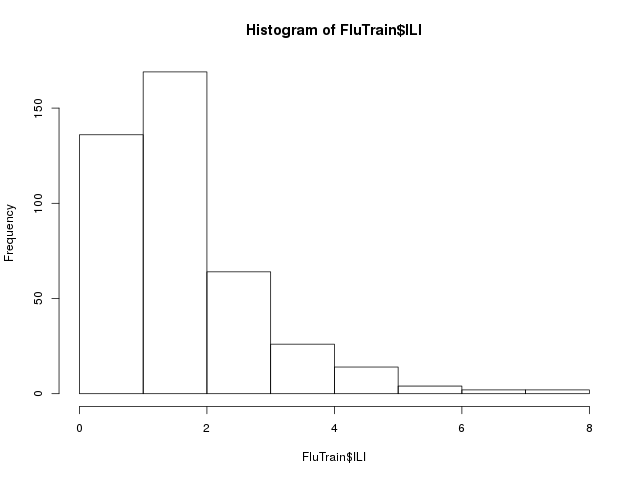
\includegraphics[width=.9\linewidth]{../graphs/ExploratoryILI.png}
\caption{\label{fig:ExploratoryILI}Histogram of the dependent variable, ILI}
\end{figure}

\subsubsection{Answer}
\label{sec-3-2-1}

Most of the ILI values are small, with a relatively small number of
much larger values (in statistics, this sort of data is called "skew
right").

\textbf{Explanation}

The histogram of ILI can be obtained with
hist(FluTrain\$ILI). Visually, the data is skew right.

\subsection{{\bfseries\sffamily DONE} Problem 1.3 - Understanding the Data (1 point possible)}
\label{sec-3-3}
When handling a skewed dependent variable, it is often useful to
predict the logarithm of the dependent variable instead of the
dependent variable itself -- this prevents the small number of
unusually large or small observations from having an undue influence
on the sum of squared errors of predictive models. In this problem, we
will predict the natural log of the ILI variable, which can be
computed in R using the log() function.

Plot the natural logarithm of ILI versus Queries. What does the plot
suggest?.

\begin{figure}[htb]
\centering
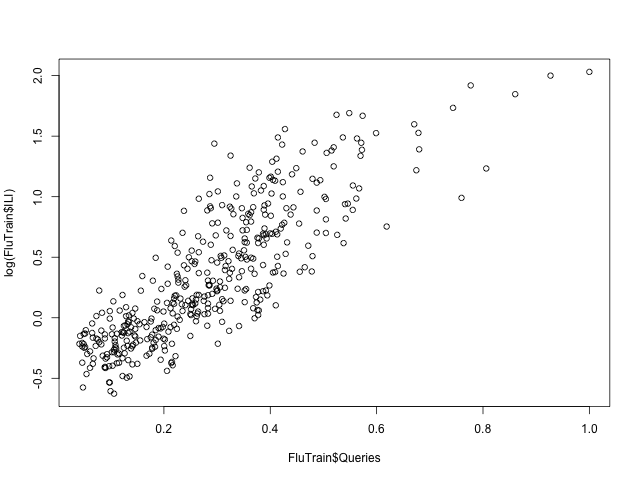
\includegraphics[width=.9\linewidth]{../graphs/LogILIvsQueries.png}
\caption{\label{fig:LogILIvsQueries}Natural logarithm of ILI versus Queries}
\end{figure}

\subsubsection{Answer}
\label{sec-3-3-1}

\textbf{Explanation}

The plot can be obtained with

plot(FluTrain\$Queries, log(FluTrain\$ILI)).

Visually, there is a positive, linear relationship between log(ILI)
and Queries.

\subsection{{\bfseries\sffamily TODO} Problem 2.1 - Linear Regression Model (1 point possible)}
\label{sec-3-4}

Based on the plot we just made, it seems that a linear regression
model could be a good modeling choice. Based on our understanding of
the data from the previous subproblem, which model best describes our
estimation problem?

\begin{minted}[]{r}
logILIReg <- lm(ILI ~ Queries, data = FluTrain)
summary(logILIReg)
\end{minted}

\begin{verbatim}
Call:
lm(formula = ILI ~ Queries, data = FluTrain)

Residuals:
     Min       1Q   Median       3Q      Max
-1.73911 -0.38816 -0.04161  0.31012  2.48517

Coefficients:
            Estimate Std. Error t value Pr(>|t|)
(Intercept)  0.01374    0.06646   0.207    0.836
Queries      5.81454    0.20352  28.570   <2e-16 ***
---
Signif. codes:  0 ‘***’ 0.001 ‘**’ 0.01 ‘*’ 0.05 ‘.’ 0.1 ‘ ’ 1

Residual standard error: 0.6546 on 415 degrees of freedom
Multiple R-squared:  0.6629,	Adjusted R-squared:  0.6621
F-statistic: 816.2 on 1 and 415 DF,  p-value: < 2.2e-16
\end{verbatim}

\subsubsection{Answer}
\label{sec-3-4-1}

\textbf{Explanation}

From the previous subproblem, we are predicting log(ILI) using the
Queries variable. From the plot in the previous subproblem, we expect
the coefficient on Queries to be positive.
% Emacs 24.4.1 (Org mode 8.2.10)
\end{document}
